\documentclass{article}
\usepackage[utf8]{inputenc}

% trees
\usepackage{tikz}
\usetikzlibrary{trees}

% arrows
\usetikzlibrary{arrows.meta}

% colors
\usepackage{color}

%\tikzset{%
   neuron missing/.style={
    draw=none,
    scale=2,
    text height=0.333cm,
    execute at begin node=\color{black}$\vdots$
  },
}

% The command \DrawNeuronalNetwork has a list as argument, each entry is a layer.
% Each entry has the form:
% Layer name/number of nodes/color/missing node (dots)/label/symbolic number
%
% * "layer name" is the name of the layer
% * "number of nodes" is the number of neurons in that layer (including the missing neuron)
% * "color" is the color of the layer
% * "missing node" denotes the index of the missing neuron, replaced by the dots
% * "label" denotes the label of the layer
% * "symbolic number" denotes the symbol that indicates how many neurons there are

\newcommand{\DrawNeuronalNetwork}[2][]{
\xdef\Xmax{0}
\foreach \Layer/\X/\Col/\Miss/\Lab/\Count [count=\Y] in {#2}
{\pgfmathsetmacro{\Xmax}{max(\X,\Xmax)}
 \xdef\Xmax{\Xmax}
 \xdef\Ymax{\Y}
}
\foreach \Layer/\X/\Col/\Miss/\Lab/\Count [count=\Y] in {#2}
{\node[anchor=south] at ({2*\Y},{\Xmax/2+0.1}) {\Layer};
 \foreach \m in {1,...,\X}
 {
  \ifnum\m=\Miss
   \node [neuron missing] (neuron-\Y-\m) at ({2*\Y},{\X/2-\m}) {};
  \else
   \node [circle,fill=\Col!50,minimum size=1cm] (neuron-\Y-\m) at
  ({2*\Y},{\X/2-\m}) {};
 \ifnum\Y=1
  \else
   \pgfmathtruncatemacro{\LastY}{\Y-1}
   \foreach \Z in {1,...,\LastX}
   {
    \ifnum\Z=\LastMiss
    \else
     \draw[->] (neuron-\LastY-\Z) -- (neuron-\Y-\m);
    \fi
    }
  \fi
 \fi
 \ifnum\Y=1
  \ifnum\m=\X
   \draw [<-] (neuron-\Y-\m) -- ++(-1,0) node [above, midway] {$\Lab_{\Count}$};
  \else
   \ifnum\m=\Miss
   \else
    \draw [<-] (neuron-\Y-\m) -- ++(-1,0) node [above, midway] {$\Lab_{\m}$};
   \fi
  \fi
 \else
   \ifnum\Y=\Ymax
    \ifnum\m=\X
     \draw [->] (neuron-\Y-\m) -- ++(1,0) node [above, midway] {$\Lab_{\Count}$};
    \else
     \ifnum\m=\Miss
     \else
      \draw [->] (neuron-\Y-\m) -- ++(1,0) node [above, midway] {$\Lab_{\m}$};
     \fi
    \fi
   \else
     \ifnum\m=1
      \node[above=0pt of neuron-\Y-\m] {$\Lab_1$};
     \fi
     \ifnum\m=\X
      \node[below=0pt of neuron-\Y-\m] {$\Lab_{\Count}$};
     \fi
   \fi
 \fi
 }
 \xdef\LastMiss{\Miss}
 \xdef\LastX{\X}
}
}
\definecolor{orange}{RGB}{253, 192, 134} % rgb(253,192,134)
\definecolor{light_orange}{RGB}{253, 192, 134} % rgb(253,192,134)

\definecolor{blue}{RGB}{37, 150, 190} % rgb(37, 150, 190)
\definecolor{light_blue}{RGB}{146, 203, 223} % rgb(146, 203, 223)

\definecolor{green}{RGB}{159, 188, 43} % rgb(159,188,43)
\definecolor{light_green}{RGB}{207, 221, 149} % rgb(207,221,149)

\definecolor{yellow}{RGB}{255, 205, 64} % rgb(255, 205, 64)
\definecolor{light_yellow}{RGB}{255, 230, 59} % rgb(255, 230, 159)

\definecolor{red}{RGB}{252, 76, 70} % rgb(252,76,70)
\definecolor{light_red}{RGB}{250, 155, 153} % rgb(250,155,153)


\definecolor{red}{RGB}{250,155,153} % rgb(250,155,153)

\definecolor{orange}{RGB}{247,187,150} % rgb(247,187,150)

\definecolor{yellow}{RGB}{246,210,152} % rgb(246,210,152)

\definecolor{blue}{RGB}{115,190,222} % rgb(115,190,222)

%python code
\usepackage{listings}

%floor 
\usepackage{mathtools}
\DeclarePairedDelimiter\ceil{\lceil}{\rceil}
\DeclarePairedDelimiter\floor{\lfloor}{\rfloor}

\title{Automated Search}
\author{}
\date{}

\begin{document}

\maketitle

\section{Problem solving agents}

Search algorithms are one of the most important areas of Artificial Intelligence.\\ 

Search algorithms are universal problem-solving techniques. They allow the AI system to efficiently find a solution to a problem among a large set of possibilities. These algorithms can be used for a variety of tasks, such as planning, decision-making, and problem-solving. They can also be used to optimize machine learning models by finding the best parameters or architecture. \\

Given that:

\begin{center}
    \begin{itemize}
        \item \textbf{Search space} is the set of possible solutions which a system may have;
        \item \textbf{Start state} is the state in which the agent is initially;
        \item \textbf{Goal state} is the state the agent needs to reach.
    \end{itemize}
\end{center}

a problem could be viewed as moving in the state space from the initial state towards a goal state. Searching is a step by step procedure to solve this kind of problem. \\

A representation of the search problem is called \textbf{search tree}. The root of the search tree is the initial state, the nodes are the other states and the solution (goal state) is among them. We don't know where the solution is in the tree, so we need to search. The choice of the node being \textbf{expanded} represents the \textbf{search strategy}. \\

\begin{itemize}
    \item a \textbf{state} is physical configuration;
    \item a \textbf{node} is a data structure part of the search tree and includes \textbf{parent, children, depth, path cost $g(n)$}. 
\end{itemize}

\begin{flushleft}
    \textbf{states} do not have parent, children and so on.
\end{flushleft}

\newpage

\section{Search strategies}

A strategy is defined by picking the order of node expansion.

\subsection{Properties of search algorithms}

\textbf{In what terms one search algorithms is better than another one?} To compare the efficiency of these algorithms we can use the following properties:

\begin{itemize}
    \item \textbf{completeness}: a search algorithm is said to be complete if for any random input it guarantees to return a solution if at least any solution exists;
    \item \textbf{optimality}: a search algorithm is said to be optimal if it is guaranteed that the solution found is the best one (lowest path cost) among other; 
    \item \textbf{Time complexity}: time complexity measures the time an algorithm takes to complete a task;
    \item \textbf{Space complexity}: space complexity measures the storage space required for an algorithm at any point during the search;
\end{itemize}

Finding the optimal solution entails proving optimality. This can be done by finding all solutions or by proving that no solution can have better cost than the one found already. In either case, at least one solution has to be found.

If there is no solution, neither an optimal nor a complete algorithm would find one of course.
\begin{equation}
    optimality\ \rightarrow completeness
\end{equation}

\begin{equation}
    !\ complete\ \rightarrow\ !\ optimal
\end{equation}

\subsection{Types of search algorithms}

Based on the search problem itself, we can classify the search strategies into:

\begin{itemize}
    \item \textbf{uninformed}: does not contain any domain knowledge such as closeness or the location of the goal; an uninformed search algorithm will examine each node of the three until it achieves the goal node;
    \item \textbf{informed}: problem information is available which can guide the search; they are based on the use of \textbf{heuristics};
\end{itemize}

Heuristic functions estimate the cost of the cheapest path from the current state (node) to the goal. An heuristic does not guarantees to find the best solution but guarantees to find a good solution in reasonable time.

Informed search algorithms are generally more efficient than uninformed search algorithms because they can focus the search process on more promising areas of the search space. However, the quality of the solution found by an informed search algorithm depends on the accuracy of the heuristic function used.

\newpage

\section{Uninformed search}

Algorithms have no additional information on the goal node other than the ones provided in the problem definition. 

\begin{center}
    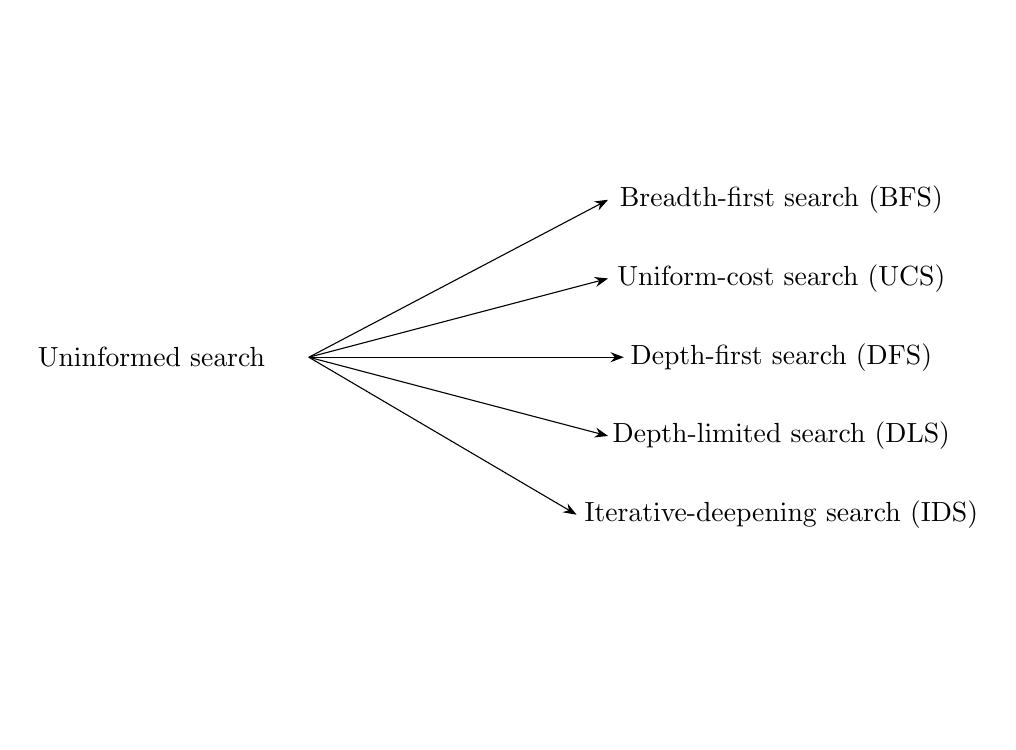
\begin{tikzpicture}
        \node[shape=circle] (A) at (0, 0) {Uninformed search};
        \node[shape=circle] (B) at (8, 2) {Breadth-first search (BFS)};
        \node[shape=circle] (C) at (8, 1) {Uniform-cost search (UCS)};
        \node[shape=circle] (D) at (8, 0) {Depth-first search (DFS)};
        \node[shape=circle] (E) at (8,-1) {Depth-limited search (DLS)};
        \node[shape=circle] (F) at (8,-2) {Iterative-deepening search (IDS)};

        \draw[-{Stealth[black]}] (2,0) -- (5.8,2);
        \draw[-{Stealth[black]}] (2,0) -- (5.8,1);
        \draw[-{Stealth[black]}] (2,0) -- (6,0);
        \draw[-{Stealth[black]}] (2,0) -- (5.8,-1);
        \draw[-{Stealth[black]}] (2,0) -- (5.4,-2);
    \end{tikzpicture}
\end{center}

\subsection{Breadth-first search (BFS)}

The tree is explored looking first at the root node, then at all its neighbors, then at the next level neighbors and so on. This process continues until all the nodes in the tree have been explored. \\

The iterative implementation uses a \textbf{queue} (\textbf{FIFO} structure). It is complete and optimal: that means that it will find the shallower solution, it it exists, with the minimum amount of actions. It finds the optimal solution in $O(b^d)$, scanning the entire tree, and occupies $O(b^d)$ of memory.

\begin{center}
    \textit{frontier = queue}
\end{center}

\newpage

\subsection{Uniform-cost search (UCS)}

Uniform-cost search \textbf{expands the node with the lowest path cost $g(n)$}. \\

Uniform-cost search uses the lowest cumulative cost to find a path from the source to the destination. Nodes are expanded, starting from the root, according to the minimum cumulative cost $g(n)$. The search is implemented using a \textbf{priority queue} with $p(n) = g(n)$.

\begin{center}
    \textit{frontier = priority queue}
\end{center}

It is complete (if each step cost $\geq \epsilon$ and optimal. t can be inefficient in situations where the cost of reaching a goal state is large, but there are also many lower-cost paths that lead to states that are not the goal state. In such cases, the algorithm may explore a large number of unnecessary states before finding the goal state, leading to a high time complexity. Additionally, if the cost function is not consistent, the algorithm may get stuck in an infinite loop.

\newpage

\subsection{Depth-first search (DFS)}

Depth-first search is a method for traversing a graph or tree data structure. The root node is visited first, the next one is chosen by going deeper into the tree/graph. This process continues until a leaf node (a node with no children) is reached, then the process backtracks to the most recent node that has unvisited children. DFS is implemented using a \textbf{stack} data structure to keep track of the nodes to be visited next (\textbf{LIFO} structure). DFS is used for tasks such as topological sorting, solving mazes and puzzles, and searching for connected components in a graph.

\begin{center}
    \textit{frontier = stack}
\end{center}

It is NOT complete since it fails in infinite-depth spaces or spaces with loops. We can easily keep track of visited nodes and avoid re-expanding them, so the algorithm can be extended to support spaces with loops, but the problems with infinite-depth spaces persist. It is NOT optimal since it could miss some shallower solution going deeper and deeper. It occupies $O(b * m)$ memory (only the current path) and finds a solution in the finite-depth space case in $O(b^m)$. 

\newpage

\subsection{Depth-limited search (DLS)}

This search is like the Depth-first search but there is a limit in the tree's depth. In this way, the search process cannot continue infinitely. If there is not a solution in the subtree considered, the algorithm will not be able to find any solution, and is therefore NOT complete. It is not optimal for the same reason. It finds a solution in $O(b^d)$ if present and occupies $O(b*l)$ memory ($l$ being the depth limit).

\newpage

\subsection{Iterative-deepening search (IDS)}

This search algorithms is nothing more than an iteration of DLS, increasing the limit at each step. It starts from $l=1$ and increases it until the shallowest solution is found. It IS complete because it finds a solution acting in a similar way of BFS, but requiring significantly less memory. The complexity is $O(b^d)$ for time and $O(b^d)$ for memory occupation. 

\subsection{Uniformed search comparison}

\begin{center}
    \begin{table}[h]
        \begin{tabular}{l | l | l | l | l}
            Search & Completeness & Optimality & Time & Space \\
            algorithm & & & complexity & complexity \\
            & & & & \\
            \hline
            & & & & \\
            Breadth-first & yes (if b is finite) & yes (if cost = 1) & $O(b^d)$ & $O(b^d)$ \\
            & & for each step & & \\
            & & & & \\
            Uniform-cost & yes (if step cost) $\geq\ \epsilon$ & yes & $O(b^{\ceil{1 + C^*/\epsilon}})$ & $O(b^{\ceil{C^*/\epsilon}})$ \\
            & & & & \\
            Depth-first & no (if domain & no & $O(b^m)$ & $O(bm)$ \\
            & is depth-infinite) & & & \\
            & & & & \\
            Depth-limited & no & no & $O(b^d)$ & $O(bl)$ \\
            & & & & \\
            Iterative-deepening & yes & yes & $O(b^d)$ & $O(bd)$
        \end{tabular}
    \end{table}
\end{center}

\begin{flushleft}
    with:
\end{flushleft}
\begin{itemize}
    \item $b$: average branching factor;
    \item $d$: depth;
    \item $l$: limit on the depth;
    \item $m$: maximum depth;
    \item $C^*$: cost of the optimal solution;
    \item $\epsilon$: least cost of a step; 
\end{itemize}

\newpage

\section{Search direction}

Search can be:

\begin{itemize}
    \item \textbf{forward} (or data driven);
    \item \textbf{backward} (or goal driven);
    \item \textbf{bidirectional} (or mixed);
\end{itemize}

An alternative approach called bidirectional search simultaneously searches forward and backwards if the problem allows it, hoping that the two searches will meet midway. The motivation is that

\begin{equation}
    b^{d/2} + b^{d/2} << b^d
\end{equation}

\begin{flushleft}
    We have a solution when the two frontiers collide. Completeness and optimality depends on the search strategies adopted.
\end{flushleft}

\newpage

\section{Informed search}

Some algorithms make use of an evaluation function $f(n)$ to decide which node to expand first. Informed search algorithms make use of an \textbf{heuristic function} $h(n)$ which estimates the cost of the cheapest path from the current node to the goal.

\begin{center}
    \begin{figure}[b!]
        \centering
        \begin{tikzpicture}
            \node[shape=circle] (A) at (0, 0) {Informed search};
            \node[shape=circle] (B) at (8, 2) {Greedy best-first search (GBFS)};
            \node[shape=circle] (C) at (8, 1) {Recursive best-first search (RBFS)};
            \node[shape=circle] (D) at (8, 0) {A*};
            \node[shape=circle] (E) at (8,-1) {Iterative deepening A* (IDA*)};
            \node[shape=circle] (F) at (8,-2) {Simplified memory-bounded A* (SMA*)};
        
            \draw[-{Stealth[black]}] (2,0) -- (5.4,2);
            \draw[-{Stealth[black]}] (2,0) -- (5.2,1);
            \draw[-{Stealth[black]}] (2,0) -- (7.7,0);
            \draw[-{Stealth[black]}] (2,0) -- (5.5,-1);
            \draw[-{Stealth[black]}] (2,0) -- (4.8,-2);
        \end{tikzpicture}
    \end{figure}
\end{center}

\newpage

\subsection{Heuristic function properties}

\begin{itemize}
    \item \textbf{Dominance}: a heuristic function $h_1(n)$ dominates another heuristic function $h_2(n)$ iff:
    \begin{equation}
        \forall n : h_1(n) \geq h_2(n)
    \end{equation}

    \item \textbf{Admissibility}: a heuristic function is admissible if it never overestimates the cost to reach the goal;

    \item \textbf{Consistency}: a heuristic function is consistent if the estimated cost to reach the goal from $n$ is not greater than the cost to reach $n'$, child of $n$, plus the estimated cost from $n'$ to the goal:

    \begin{equation}
        h(n) \leq c(n,n') + h(n')
    \end{equation}

\begin{center}
    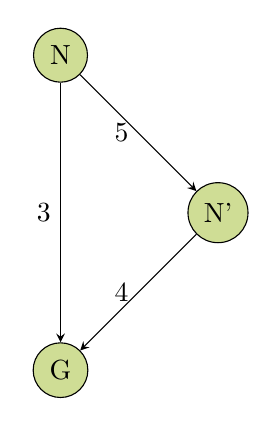
\begin{tikzpicture}
        \node[shape=circle, draw=black, fill=light_green] (A) at (0,0) {N};
        \node[shape=circle, draw=black, fill=light_green] (B) at (2,-2) {N'};
        \node[shape=circle, draw=black, fill=light_green] (C) at (0,-4) {G} ;

    \begin{scope}[every edge/.style={draw=black}]
        \draw [-stealth](A) edge node[left] {$5$} (B);
        \draw [-stealth](A) edge node[left] {$3$} (C);
        \draw [-stealth](B) edge node[left] {$4$} (C);
    \end{scope}
        
    \end{tikzpicture}
\end{center}    
\end{itemize}

\subsection{Combination of heuristics}

What if we have several heuristics not dominating each other? \\

Let $h_1, ..., h_m$ be a collection of such heuristics, define:

\begin{equation}
    h(n) = max (h_1(n), ..., h_m(n))
\end{equation}

$h$ is admissible and dominates $h_1, ..., h_m$.

\subsection{Building an heuristic}

Admissible heuristics can be derived from the exact solution cost of a relaxed version of the problem (relaxed problem: some of the constraints are removed). Problem relaxation is a good way to find a good heuristic. \\

\newpage

\subsection{Greedy best-first search (GBFS)}

Greedy BFS uses the following evaluation function $f(n) = h(n)$, which is just the heuristic function $h(n)$, that estimates the closeness of $n$ to the goal. Hence, greedy BFS tries to expand the node that is thought to be closest to the goal, without taking into account previously gathered knowledge (i.e. $g(n)$). \\

It has time complexity $O(b^m)$ where $b$ is the branching factor (the average number of children per node) and $m$ is the maximum depth of the search space, and space complexity $O(b^m)$ (it keeps all the nodes in memory). Can get stuck in loops and it is therefore not complete. Not accounting for $g(n)$ it may not always find the shortest path. \\

If the heuristic function is not accurate or consistent, it may lead to suboptimal solutions or even get stuck in loops. A good heuristic on the other hand can give dramatic improvements. 

\newpage

\subsection{Dijkstra's algorithm}

Dijkstra's algorithm allows us to calculate the shortest path between a set of nodes. It works on weighted graphs and can find the shortest paths from the start node to all the other nodes on the graph. The shortest path is the sequence of nodes, in the order they are visited, which results in the minimum cost to travel between the start and the end node. \\

\begin{flushleft}
    $A^*$ is basically Dijkstra's algorithm for two nodes and with an heuristic function.
\end{flushleft}

\subsection{$A^*$ search}

The most common informed search algorithm is $A^*$.

$A^*$ uses a combination of a heuristic function and a cost function $f(n) = g(n) + h(n)$ to evaluate the potential path and determine the best one to take. The heuristic function $h(n)$ estimates the cost of the cheapest path from the current node to the goal node, while the cost function $g(n)$ measures the actual cost of the path from the starting node to the current node. $A^*$ repeatedly selects the node with the lowest estimated total cost $f(x) = g(x) + h(x)$ until it reaches the goal node. \\

$A^*$ is guaranteed to find the shortest path if heuristic function is admissible (never overestimate the real distance) and consistent (the distance from current node to the goal node is always less than from neighbor to goal node through current node) but GBFS may not. \\

$A^*$ is complete, unless there are infinitely many nodes with $f < f(G)$ (estimated cost of the goal).
It is also optimal. The problem is that the spacial complexity is exponential $O(b^m)$ as in GBFS. \\




\begin{flushleft}
    Cons: the memory necessary to store the frontier may be exponential.
\end{flushleft}

\newpage

\subsection{F-countours}

An f-contour represents the set of nodes that have the same estimated total cost $(f(x) = g(x) + h(x))$ in the pathfinding process. In other words, it is the boundary between the set of nodes that have been expanded (visited) and the set of nodes that have not yet been expanded.

F-contour is important in $A^*$ algorithm as it can help to prune search space by considering only nodes that are on the current f-contour. It can also help to identify the suboptimal solution and discard it, as well as to identify the optimal solution faster.

\begin{center}
    Contour $i$ has all nodes with $f = f_i$, where $f_i < f_{i+1}$
\end{center}

\subsection{Iterative-deepening $A^*$ ($IDA^*$)}

$IDA^*$ gives us the benefits of $A^*$ (completeness and optimality) without the requirement to keep all reached states in memory, at a cost of visiting some states multiple times; it is, for this reason, very commonly used for problems that do not fit in memory. \\

Each iteration exhaustively searches an \textbf{f-contour}, finds a node just beyond that contour and uses that node's cost as the next contour value. We can limit this way memory consumption and thus have linear spacial complexity $O(bm)$. This is because it uses a limited amount of memory at each iteration. It does not need to store the whole search tree as $A^*$ does.

\newpage

\subsection{Recursive best-first search (RBFS)}

\textbf{RBFS is a valid alternative to $IDA^*$}

Recursive best-first search stores the f-value of the unexpanded nodes and goes depth-first until the f of the current node does not become worse of the one of the previous alternatives. Whenever the cost of the current node exceeds that of some other node in the previously expanded portion of the tree, the algorithm backs up to their deepest common ancestor, and continues the search down the new path. \\

\subsection{RBFS vs $IDA^*$}

Both algorithms have their own advantages and disadvantages depending on the problem you are trying to solve. $IDA^*$ is more space efficient than RBFS, but RBFS is more flexible in terms of the heuristic function it can use. \\

In general, $IDA^*$ is considered to be more efficient than RBFS when the heuristic function is consistent and admissible, and when the branching factor of the search space is moderate or low. \\

In contrast, RBFS is considered to be more efficient than $IDA^*$ when the heuristic function is highly inconsistent or inadmissible, and when the branching factor of the search space is high.

\subsection{$SMA^*$}

\begin{center}
    $IDA^*$ uses too little memory: only the current f-value;
    $RBFS$ uses too little memory: only the cost of the nodes in the depth first search are recorded;
\end{center}

Simplified memory bounded $A^*$ can use all the available memory for the search. It behaves like $A^*$ till there is memory available. When a new node needs to be generated and the memory is full, the node in memory with the highest f-value is discarded while keeping its cost in the parent node. A discarded node will be re-generated only when all the other paths are worse than the forgotten node.

\newpage

\section{Local search}

Local search algorithms operate by searching from a start state to neighbouring states, without keeping track of the paths, nor the set of states that have been reached. That means they are not systematic: they might never explore a portion of the search space where a solution actually resides. \\

They have two key advantages:

\begin{itemize}
    \item they use very little memory;
    \item they can often find a solution in large or infinite state spaces for which systematic algorithms are unsuitable.
\end{itemize}

\subsection{Hill climbing}

Hill climbing is a heuristic optimization algorithm that attempts to find the local maximum of a function. It starts at a randomly chosen point on the search space and repeatedly moves in the direction of increasing value until no more such steps can be taken. Hill climbing can be useful for solving optimization problems, but it can also get stuck in many scenarios: \\

\begin{itemize}
    \item local maxima/minima: a peak that is higher/lower than any of its neighbors but lower/higher than the global maxima/minima;
    \item ridges result in a sequence of local maxima/minima that is very difficult for greedy algorithm to navigate;
    \item plateaus: a flat area of the state-space;
\end{itemize}

\begin{center}
    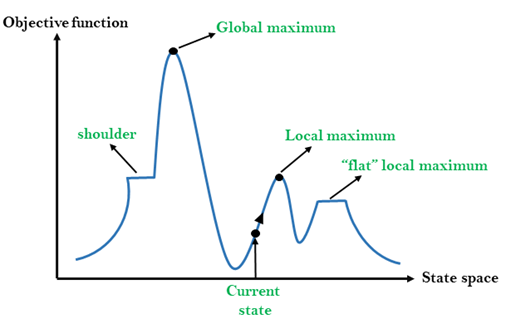
\includegraphics[width=0.8\textwidth]{images/hill-climbing.png}    
\end{center}

To avoid getting stuck in local maxima, variations of the algorithm such as simulated annealing and genetic algorithms can be used.

\newpage

\subsection{Simulated annealing (SA)}

Simulated Annealing is a probabilistic algorithm for global optimization that is often used to find an approximate solution to difficult optimization problems. The algorithm models the process of heating a material and then slowly cooling it down to find a state close to the global minimum energy state.

The basic process of the algorithm is as follows:

\begin{enumerate}
    \item Start with an initial solution (e.g., a randomly generated state);
    \item Generate a new solution by making small random changes to the current solution;
    \item Calculate the energy difference between the new solution and the current solution;
    \item Decide whether to accept the new solution as the current solution, based on a probability that depends on the energy difference and a temperature parameter.
    \item Repeat steps 2-4 until the temperature parameter has cooled to a low value or a stopping criterion is met.
\end{enumerate}

The time complexity of the SA algorithm is generally considered to be $O(kT^n)$, where $k$ is the number of iterations at a given temperature, $T$ is the number of temperature values, and $n$ is the number of variables in the problem. The space complexity is $O(n)$.

\newpage

\subsection{Random restart vs Simulated annealing}

Random restart and simulated annealing are both techniques used to improve the performance of hill climbing algorithms, which are optimization algorithms that try to find the maximum or minimum value of a function by making incremental changes to the current solution and accepting the change if it improves the solution. \\

Random restart is a technique where the algorithm starts from a randomly generated solution and repeatedly applies the hill climbing algorithm until it finds a satisfactory solution. The idea behind random restart is that by starting from different initial solutions, the algorithm has a higher chance of escaping local optima and finding the global optimum. \\

Simulated Annealing starts from an initial solution and then generates a new solution that is randomly different from the current one. The algorithm will accept the new solution if it is better than the current one, otherwise, it will accept it with a probability that decreases as the number of iterations increases. The idea behind this is that the algorithm will not get stuck in a local optimum but it will be able to explore a wider range of solutions by allowing some bad moves.

In summary, random restart is a technique where the algorithm starts from different initial solutions, Simulated Annealing is a technique that allows bad moves early in the optimization process, but reduces the likelihood of bad moves as the optimization process progresses.

\newpage

\subsection{Local beam search (LBS)}

Each iteration, LBS generates a set of new states from the current beam, and then selects the best $k$ states from the combination of the current beam and the new states to form the next beam. The process repeats until a goal state is found or a certain stopping criterion is met. \\

\begin{center}
The problem is that the states converge in the same region of the search space. \\     
\end{center}

LBS can easily get stuck in local optima. Because LBS only generates new states from the states in the current beam, it has a limited view of the search space and may miss global optima that are outside of its current beam. This can lead to the algorithm converging on a suboptimal solution, rather than the true optimal solution.

\subsection{Genetic algorithms}

Genetic algorithms work by simulating the logic of Darwinian selection. 

Genetic algorithms starts by generating an initial population (random strings). 

\begin{enumerate}
    \item This \textbf{initial population} consists of all the probable solutions to the given problem.

    \item The \textbf{fitness function} helps in establishing the fitness of all the individuals in the population. It assigns a fitness score to each of them, which further determines the probability of being chosen for reproduction. The higher the fitness score, the higher the changes of being selected.

    \item In the \textbf{selection phase}, individuals are selected and then arranged in pairs of two to enhance reproduction. The genetic algorithm uses the \textbf{fitness proportionate selection technique} to ensure that useful solutions are used for recombination.

    \item The \textbf{reproduction phase} involves the creation of the child population. The two main operators in this phase include crossover and mutation.

    \begin{itemize}
        \item \textbf{Crossover}: this operator swaps the genetic information of the two parents to produce the offspring; the child population is of equal size as the parent population.
        \item \textbf{Mutation}: this operator adds new genetic information to the new child population; this is achieved by flipping some bits in the chromosomes. Mutation \textbf{solves the problem of local minimum} and enhances diversification.
    \end{itemize}

    \item \textbf{Genetic replacement} takes place next: the old population is replaced with the new child population. The new population consists of higher fitness score than the old population.

    \item If a \textbf{stopping criterion} is met, we could terminate (threshold in fitness).
\end{enumerate}

\end{document}
